% !TEX program = xelatex
\documentclass[10pt,letterpaper]{article}

% ---------- FONTS ---------------------------------------------
\usepackage{fontspec}
\IfFontExistsTF{Roboto}
    {\setmainfont{Roboto}}
    {\IfFontExistsTF{Helvetica Neue}
        {\setmainfont{Helvetica Neue}}
        {\setmainfont{Latin Modern Sans}}}

% ---------- GEOMETRY ------------------------------------------
\usepackage[
  letterpaper,
  left=0.55in, right=0.55in,
  top=0.8in,  bottom=0.8in
]{geometry}

% ---------- COLOURS & GRAPHICS --------------------------------
\usepackage[dvipsnames,svgnames,x11names]{xcolor}
\definecolor{primary}{HTML}{004A99}
\definecolor{accent}{HTML}{E6F4FF}

\usepackage{graphicx}
\usepackage{tikz}
\usetikzlibrary{calc}

% ---------- LAYOUT HELPERS ------------------------------------
\usepackage{paracol}
\columnratio{0.32}
\setlength{\columnsep}{0.25in}

\usepackage[most]{tcolorbox}
\tcbset{colback=accent, colframe=accent, boxrule=0pt, sharp corners}

\usepackage{enumitem}
\setlist[itemize]{noitemsep,topsep=0pt,leftmargin=*}

\usepackage{sectsty}
\allsectionsfont{\color{primary}\bfseries\uppercase}
\subsectionfont{\color{primary}\bfseries}
\renewcommand{\thesection}{}

% ---------- UTILITIES -----------------------------------------
\newcommand{\cvName}[1]{\vspace*{0.3in}\textbf{\LARGE #1}}
\newcommand{\cvHeadline}[1]{\par\smallskip\textit{#1}}
\newcommand{\cvHr}{\vspace{0.5\baselineskip}\hrule height 1pt\color{primary}\vspace{0.7\baselineskip}}

% ==============================================================
\begin{document}\small
\begin{paracol}{2}

% ================== SIDEBAR ====================================
\begin{leftcolumn}
\begin{center}
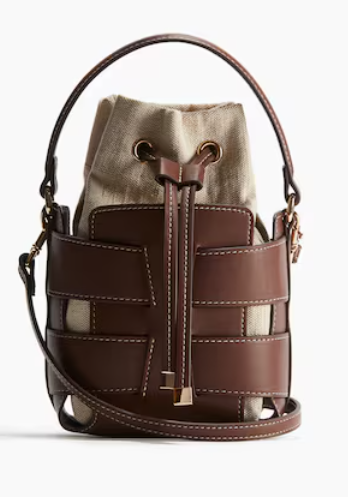
\includegraphics[width=1.6in,height=1.6in,keepaspectratio]{ea981acc637847edbc104f1e9916bac5.png}
\end{center}

\vspace{0.6in}

\cvName{Pape Saliou FALL}
\cvHeadline{Data Scientist}
\cvHr

\section*{Contact Information}
0753481453\\
papesalioufall2@gmail.com\\
\textit{LinkedIn :}\,\\ % lien non communiqué
Paris, Île-de-France, France\\
\textit{Site web :}\,

\cvHr
\section*{Languages}
Français (natif)\\
Anglais (courant)

\cvHr
\section*{Key Skills}
\begin{itemize}
  \item Python, R, SQL
  \item Machine Learning (scikit-learn, XGBoost), Statistiques avancées
  \item Deep Learning (TensorFlow, Keras), NLP (spaCy, transformers)
  \item Data Visualisation (Tableau, Power BI, Matplotlib, Seaborn)
  \item Big Data (PySpark, Hadoop), Cloud Computing (AWS, GCP)
  \item Git / CI-CD, Docker \& Kubernetes
\end{itemize}

\cvHr
\section*{Hobbies}
Lecture de romans de science-fiction\\
Basketball\\
Vulgarisation scientifique
\end{leftcolumn}

% ================== MAIN COLUMN ================================
\begin{rightcolumn}
\section*{Professional Summary}
Data Scientist titulaire d’un Master 2 en Data Science de Sorbonne Université, doté d’une solide expérience en modélisation prédictive, traitement du langage naturel et visualisation de données. Habitué à collaborer avec des équipes pluridisciplinaires pour transformer des données hétérogènes en informations exploitables et en produits data à forte valeur ajoutée. Passionné par l’optimisation de la prise de décision grâce à l’IA et l’apprentissage automatique.

\vspace{0.5in}
\section*{Work Experience}

% ---------- Prepaya ------------------------------------------------
\begin{tcolorbox}
  \begin{minipage}[t]{0.48\linewidth}
    Jan 2022 --\\
    \textbf{Prepaya, Paris — Data Scientist}\\
    \begin{itemize}
      \item Collecte, nettoyage et intégration de plus de 30 M de lignes de données transactionnelles.
      \item Développement de modèles de détection de fraude (Random Forest, XGBoost) améliorant la précision de 18 \%.
      \item Mise en production des modèles via des API REST (FastAPI) et déploiement sur AWS (SageMaker).
      \item Implémentation d’un pipeline d’entraînement automatisé via GitLab CI-CD, réduisant le temps de mise à jour de 40 \%.
      \item Création de tableaux de bord interactifs sous Tableau pour le suivi des KPI métier.
      \item Formation et accompagnement de 4 data analysts sur les bonnes pratiques de ML engineering.
    \end{itemize}
  \end{minipage}\hfill
  \begin{minipage}[t]{0.48\linewidth}\raggedleft
    Jun 2023
  \end{minipage}
\end{tcolorbox}

\vspace{0.5in}
\section*{Education}
\begin{tcolorbox}[colback=white,boxrule=1pt,colframe=primary]
\textbf{Master 2 — Data Science}\\
Sorbonne Université \hfill 2022–2023
\end{tcolorbox}

\begin{tcolorbox}[colback=white,boxrule=1pt,colframe=primary]
\textbf{Licence — Mathématiques \& Informatique}\\
Université Cheikh Anta Diop \hfill 2018–2021
\end{tcolorbox}

\section*{Certifications}
\begin{itemize}
  \item TensorFlow Developer Certificate — TensorFlow \hfill Oct 2023
  \item Google Cloud Professional Data Engineer — Google Cloud \hfill Jun 2024
\end{itemize}

\end{rightcolumn}
\end{paracol}
\end{document}